\documentclass[dvipdfmx]{jarticle}
\pagestyle{empty}
\usepackage{tikz}
\usetikzlibrary{calc,shapes}
\begin{document}
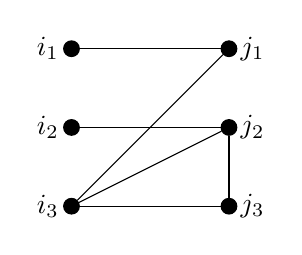
\begin{tikzpicture}
\node[draw,circle,inner sep=2pt,fill=black] (I1) at (0,0) {};
\node at ($(I1)+(-0.3,0)$) {$i_1$};
\node[draw,circle,inner sep=2pt,fill=black] (J1) at (2,0) {};
\node at ($(J1)+(0.3,0)$) {$j_1$};
\node[draw,circle,inner sep=2pt,fill=black] (I2) at (0,-1) {};
\node at ($(I2)+(-0.3,0)$) {$i_2$};
\node[draw,circle,inner sep=2pt,fill=black] (J2) at (2,-1) {};
\node at ($(J2)+(0.3,0)$) {$j_2$};
\node[draw,circle,inner sep=2pt,fill=black] (I3) at (0,-2) {};
\node at ($(I3)+(-0.3,0)$) {$i_3$};
\node[draw,circle,inner sep=2pt,fill=black] (J3) at (2,-2) {};
\node at ($(J3)+(0.3,0)$) {$j_3$};
\path[-] (I1) edge (J1) (I2) edge (J2) (I3) edge (J3);
\path[-] (J2) edge (J3) (I3) edge (J2) (J1) edge (I3);
\end{tikzpicture}
\end{document}